\subsection{Enunciado}
El problema del viajante de comercio ya se ha comentado y utilizado en la práctica sobre
algoritmos voraces, donde se estudiaron métodos de este tipo para encontrar soluciones razonables (no óptimas necesariamente) a este problema. 
Si se desea encontrar una solución óptima es necesario utilizar métodos más potentes (y costosos), 
como la vuelta atrás y la ramificación y poda, que exploren el espacio de posibles soluciones de forma más exhaustiva.

Así, un algoritmo de vuelta atrás comenzaría en la ciudad $1$ (podemos suponer sin pérdida
de generalidad, al tratarse de encontrar un tour, que la ciudad de inicio y fin es esa ciudad) e
intentaría incluir como parte del tour la siguiente ciudad aún no visitada, continuando de este
modo hasta completar un tour. Para agilizar la búsqueda de la solución se deben considerar como
ciudades válidas para una posición (ciudad actual) sólo aquellas que satisfagan las restricciones
del problema (en este caso ciudades que aún no hayan sido visitadas). Cuando para un nivel
no queden más ciudades válidas, el algoritmo hace una vuelta atrás proponiendo una nueva
ciudad válida para el nivel anterior.

Para emplear un algoritmo de ramificación y poda es necesario utilizar una cota inferior:
un valor menor o igual que el verdadero coste de la mejor solución (la de menor coste) que se
puede obtener a partir de la solución parcial en la que nos encontremos.

Una posible alternativa sería la siguiente: como sabemos cuáles son las ciudades que faltan
por visitar, una estimación optimista del costo que aún nos queda será, para cada ciudad, el
coste del mejor (menor) arco saliente de esa ciudad. La suma de los costes de esos arcos, más
el coste del camino ya acumulado, es una cota inferior en el sentido antes descrito.

Para realizar la poda, guardamos en todo momento en una variable $C$ el costo de la mejor
solución obtenida hasta ahora (que se utiliza como cota superior global: la solución óptima
debe tener un coste menor o igual a esa). Esa variable puede inicializarse con el costo de la
solución obtenida utilizando un algoritmo voraz (como los utilizados en la práctica $2$). Si para
una solución parcial, su cota inferior es mayor que $C$ entonces se puede realizar la poda.

Como criterio para seleccionar el siguiente nodo que hay que expandir del árbol de búsqueda
(la solución parcial que tratamos de expandir), se empleará el criterio LC o ``más prometedor".
En este caso consideraremos como nodo más prometedor aquel que presente el menor valor de
cota inferior. Para ello se debe de utilizar una cola con prioridad que almacene los nodos ya
generados (nodos vivos).

Además de devolver el costo de la solución encontrada (y en su caso el tour correspondiente),
se deben de obtener también resultados relativos a complejidad: número de nodos expandidos,
tamaño máximo de la cola con prioridad de nodos vivos, número de veces que se realiza la poda
y el tiempo empleado en resolver el problema.

Las pruebas del algoritmo pueden realizarse con los mismos datos empleados en la práctica
$2$ (teniendo en cuenta que el tamaño de problemas que se pueden abordar con estas técnicas es
mucho más reducido que con los métodos voraces). La visualización de las soluciones también
puede hacerse de la misma forma que en la práctica $2$ (usando gnuplot).

\subsection{Explicación}



\subsection{Eficiencia}



\subsection{Comparativa}
Comparamos los tiempos gastados con las diferentes formas de calcular cotas inferiores para poda.

Las diferentes funciones para conseguir una cota inferior hacen que en un mismo mapa
el algoritmo de ramificación y poda varíe. 
Estas variaciones se traducen en los nodos expandidos, la mayor cola de nodos vivos, la cantidad de
cortes que ha hecho cada uno y el tiempo.


\subsubsection{Cortes producidos}
Empecemos con la cantidad de cortes producidos. Esta información puede no ser representativa de la
magnitud real de los cortes aplicados. Dados dos algoritmos $X,Y$ que han hecho $x_i,y_i$ cortes
respectivamente con $x_1>y_1$ no nos está diciendo que el primero sea más rapido.
El primer algoritmo podría haber recorrido más nodos y hacer los cortes en niveles del árbol más profundos. 

Como esta gráfica solamente tiene en cuenta el número si el primer algoritmo ha podido 
cortar muchos nodos pero el segundo hacer solamente un corte que sea mejor que todos los cortes
anteriores por haberse hecho en un nivel superior.
 
\begin{figure}[H]
    \centering
%    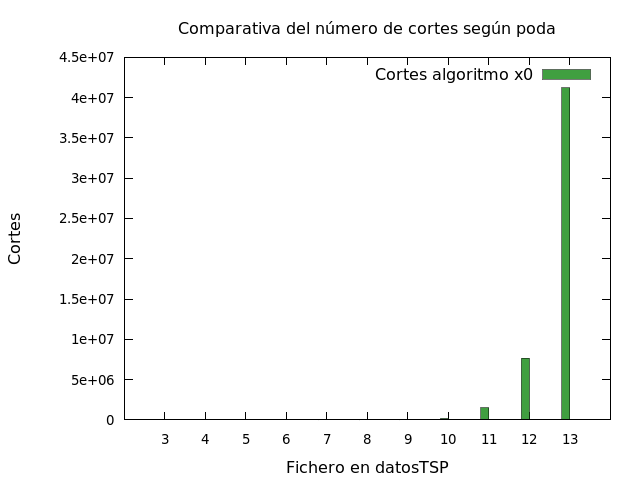
\includegraphics[scale=0.75]{../TSP/Graficas/graficaCortes.png}
    \caption{Cortes efectuados}
\end{figure}


\subsubsection{Colas con prioridad}
A continuación exponemos el mayor tamaño alcanzado por la cola con prioridad.
Esta información nos puede dar una idea de lo bueno que es nuestro algoritmo para el cálculo
de una cota inferior, es un dato mucho más valioso que la cantidad de cortes efectuados.

En los algoritmos usados nos es útil este dato, por ser algoritmos que solamente difieren en
la función de la cota inferior. Hay versiones de ramificación y poda para el problema del viajante
de comercio que no usan por ejemplo la aproximación greedy inicial, por lo que ha podido 
sobrecargar la cola con prioridad mientras busca la primera solución con la que podará después.

\begin{figure}[H]
    \centering
%    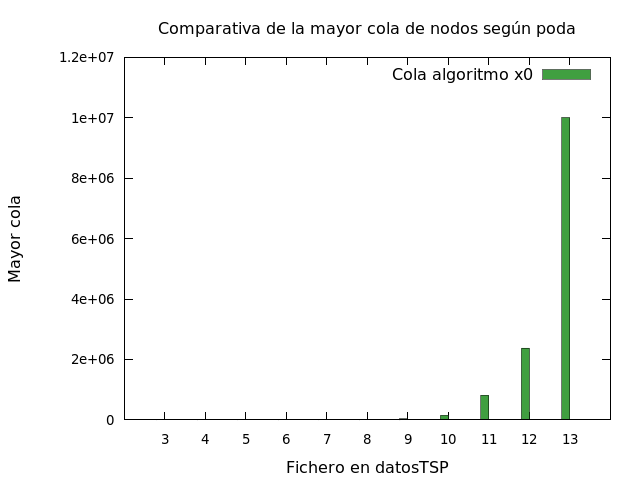
\includegraphics[scale=0.75]{../TSP/graficaColaMaxima.png}
    \caption{Cola con prioridad más grande}
\end{figure}


\subsubsection{Nodos procesados}
Otro dato interesante son los nodos que ha procesado cada algoritmo, pero esto no nos asegura
que tarde menos tiempo, ya que un algoritmo con más nodos expandidos que otro ha podido usar una
función para calcular las cotas inferiores demasiado costosa.
\begin{figure}[H]
    \centering
%    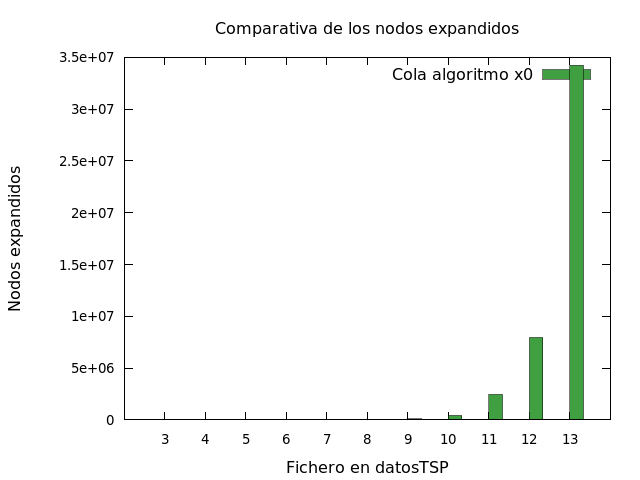
\includegraphics[scale=0.75]{../TSP/graficaNodos.png}
    \caption{Nodos expandidos}
\end{figure}



\subsubsection{Tiempos}
Todos estos datos son interesantes académicamente, pero en la práctica el tiempo es el dato
que mayor peso tendrá (además del uso de memoria) para elegir el algoritmo más eficiente o 
decantarnos por una alternativa greedy.
\begin{figure}[H]
    \centering
%    \includegraphics[scale=0.75]{../TSP/graficaTiempos0.png}
    \caption{Tiempo algoritmo 1 y su ajuste}
\end{figure}


\begin{figure}[H]
    \centering
%    \includegraphics[scale=0.75]{../TSP/graficaTiempos1.png}
    \caption{Tiempo algoritmo 2 y su ajuste}
\end{figure}


\begin{figure}[H]
    \centering
%    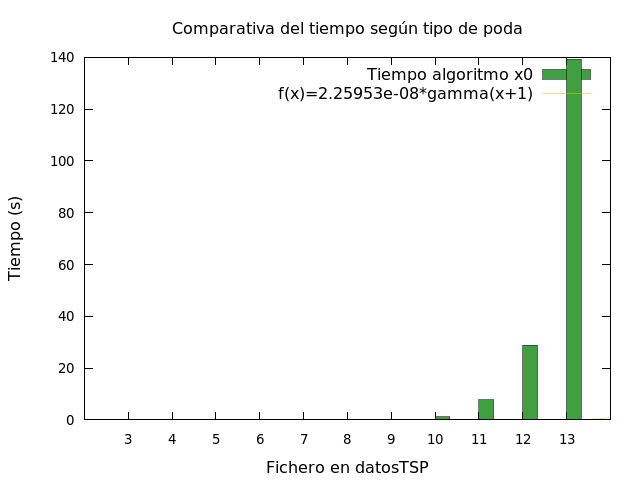
\includegraphics[scale=0.75]{../TSP/graficaTiempos.png}
    \caption{Comparativa de tiempos}
\end{figure}



\subsection{Conclusión}
Aunque los algoritmos de ramificación y poda nos aseguraran la optimalidad a problemas con
tiempos de ejecución exponenciales ahorrándonos pasos, no resultan prácticos cuando el tamaño
del problema crece. Los algoritmos greedy estudiados anteriormente nos pueden dar una aproximación
más que razonable para el problema.